\documentclass{beamer}

%\usepackage{listings}
%\usepackage[francais]{babel}
\usepackage[T1]{fontenc}
\usepackage[utf8]{inputenc}
%\usepackage{MyriadPro}
\usepackage{cabin}
\usepackage{graphicx}
\usepackage{array}
\usepackage{tikz}
\usetikzlibrary{positioning, backgrounds, shapes, chains, decorations.pathmorphing}
\usepackage{amsmath,amsthm,amssymb}  
\usepackage{stmaryrd}
%\usepackage{mdsymbol}
\usepackage{MnSymbol}
\usepackage{xcolor}
\usepackage{verbatim}
\usepackage{array}
%\usepackage{csquotes}


\useoutertheme{infolines}

\newcommand{\hidden}[1]{}

%colors
\definecolor{darkgreen}{rgb}{0,0.5,0}
\usebeamercolor{block title}
\definecolor{beamerblue}{named}{fg}
\usebeamercolor{alert block title}
\definecolor{beamealert}{named}{fg}


%\newcommand{\prop}{\textsc{\textrm{prop}}}
%\newcommand{\leftscopesign}{\raisebox{-0.75ex}{\scalebox{1.3}{$\cdot$}}\mid{}}
%\newcommand{\rightscopesign}{ {} \mid {\raisebox{-0.75ex}{\scalebox{1.3}{$\cdot$}}}}

%\newcommand{\plusl}[2]{#2\mathrel{\in_{\leftscopesign}}#1}
%\newcommand{\plusr}[2]{#2\mathrel{\in_{\rightscopesign}}#1}

%\newcommand{\dom}{\sqsubset}

%\newcommand{\ldom}{\mathrel{\dom_{\leftscopesign}}}

%\newcommand{\rdom}{\mathrel{\dom_{\rightscopesign}}}

%\newcommand{\wdom}{\trianglelefteq}

%\newcommand{\wldom}{\mathrel{\wdom_{\leftscopesign}}}

%\newcommand{\wrdom}{\mathrel{\wdom_{\rightscopesign}}}


\renewcommand{\colon}{\!:\!}


\newcommand\paraitem{%
 \quad
 \makebox[\labelwidth][r]{%
 \makelabel{%
 \usebeamertemplate{itemize \beameritemnestingprefix item}}}\hskip\labelsep}


\begin{document}

\title{Introduction to Bayesian Inference} 
\author[Antoine Venant]{Christoph Teichmann \and Antoine Venant}
%\institute{UDS COLI}
\date{\today}
\maketitle


\begin{frame}
  \frametitle{The Bayesian way of life}

 % \begin{itemize}
 % \item Let us assume there is a problem you want solve (generating text, infering a grammar, identifying distinct topics in a text), summarizing...)
  %\end{itemize}
  %\begin{block}{the Bayesian way of solving your problem}
    \begin{enumerate}
    \item<1-> Find a dataset "relevant" to your problem.
    \item<2-> Reduce your problem to estimating the distribution of some variable quantity of interest $X$.
    \item<3-> Build a {\bf joint prior probabilistic model} $p(X,Y)$ describing {\bf both} the data $O$ and the quantity $X$ you want to estimate.
    \item<4->[\alert{$\rightarrow$}]\alert{Obviously, the data and quantity of interrest should {\bf not} be independent and step 3 should reflect that fact!}
    \item<5-> Condition on all observed data $o$, and get a \textbf{posterior} distribution for $X$: $p(X \mid O=o)$.
    \item<6-> (Ideally) Assert how fit your model it, critize it and make a more realistic one.
    \item<7-> Use the posterior distribution of $Y$ to solve your problem.
    \end{enumerate}
  %\end{block}
\end{frame}

\begin{frame}
  \frametitle{A toy example: Bayesian dating service.}
  \begin{exampleblock}{Problem}
    In order to build an automatic online dating service, we would like to assess a \emph{matching score} between two registered users, as a basis for the system to determine whether it should propose this two users a date with each other. The score should be a real bumber ranging between 0 and 1.
  \end{exampleblock}
  \begin{exampleblock}{Data}
    When registering to the dating website, each of the two user answered the same set of $n$ multiple choice questions, and we dispose of these answers. Our data look like:
    \begin{tabular}{|l|l|l|}
      \hline
      $Q$ & ans. User 0 & ans. User 1\\
      \hline
      $Q_1$ & $a)$ & $b)$\\
      $Q_2$ & $c)$ & $c)$\\
      \vdots & \vdots & \vdots\\
      $Q_n$ & $a)$ & $d)$\\
      \hline
    \end{tabular}\\
    (\emph{e.g.}: $Q_1:$ \emph{You prefer a)a good movie, b)a nice book, c)a delicious meal.}) 
  \end{exampleblock}
\end{frame}

\begin{frame}
  \frametitle{Simplified data}
  \begin{itemize}
  \item To achieve maximal simplicity, we will not use the particular content of questions.
  \item We will use only the information of whether the two users' answers for a given question are the same or not.
  \item We thus extract a simplified dataset as follows:\\
    \begin{minipage}{0.48\linewidth}
      \begin{tabular}{|l|l|l|}
        \hline
        $Q$ & ans. User 0 & ans. User 1\\
        \hline
        $Q_1$ & $a)$ & $b)$\\
        $Q_2$ & $c)$ & $c)$\\
        \vdots & \vdots & \vdots\\
      $Q_n$ & $a)$ & $d)$\\
        \hline
      \end{tabular}
    \end{minipage}
    \begin{minipage}{0.05\linewidth}
      $\Rightarrow$
    \end{minipage}
    \begin{minipage}{0.2\linewidth}
      \begin{tabular}{|l|l|}
        \hline
        $Q$ & Match\\
        \hline
        $Q_1$ & no\\
        $Q_2$ & yes\\
        \vdots & \vdots\\
        $Q_n$ & no\\
        \hline
      \end{tabular}
    \end{minipage}
  \end{itemize}
\end{frame}

\begin{frame}{First step: target and observations as random variables}
  \begin{itemize}
  \item Assume an underlying probability space $\langle \Omega, p \rangle$.
  \item Our problem reduces to estimating the distribution of a \emph{matching score} random variable $\Phi: \Omega \mapsto [0, 1]$ after observing the answers made by both users.
  \item Observed data is represented as a sequence $\langle o_1, \dots o_n \rangle \in \{0,1\}^n$
  \item $o_n = 1$ means that both users choosed the same answer to the $n^\textnormal{th}$ question of the questionaire, $o_n = 0$ means that they did not.
  \item Accordingly, assume that the observed data is in fact one outcome of a random vector $O: \Omega \mapsto \{0, 1\}^n$. Equivalently, we can see $O$ as a vector of random variables $(O_1, \dots, O_n)$ where  $(O_i: \Omega \mapsto \{0,1\}$).
  \end{itemize}
    
\end{frame}

\begin{frame}{Second step: build the joint Model}
  \begin{itemize}
  \item So far we only said ``there exist some joint distribution''. Did not precise which one.
  \item Idea: assume that both users answers each question independently of others questions, and that probability of choosing matching answer equals the\emph{matching score}.
  \item This translates into: \[ p(O = (o_1, \dots o_n) \mid \Phi = \phi) = \phi^\alpha (1-\phi)^{n-\alpha} \] where $\alpha = \Sigma_{i=1}^n o_i$
  \item We also need to set a prior probability on $\Phi$. Simply assume it uniform on $[0,1]$: for $I \subseteq [0,1]$ \[P(\Phi \in I) = \int_I 1 dx\]
    (for instance $P(\Phi \le 1/2) = \int_o^{1/2} 1 dx =  [x^2/2]^{1/2}_{0} = 1/2$)
  \end{itemize}
\end{frame}

\begin{frame}{Mixing continuous and discrete models}
  \begin{alertblock}{Not so obvious:}
    \begin{itemize}
    \item $\forall \phi \in [0,1]\, P(\Phi = \phi) = \int_\phi^\phi 1 dx = 0$.
    \item So shouldn't $P(o \mid \Phi = \phi) = \frac{P(o, \Phi=\phi)}{P(\Phi=\phi)}$ be undefined if $P(\Phi = \phi)=0$?
    \item So far, no {\bf full} model: what is for instance $P(O = (o_1,\dots o_n))$?
    \end{itemize}
  \end{alertblock}

  \begin{block}{Short answer:}
    \begin{itemize}
    \item True that 'classic' conditioning does not define $P(o \mid \Phi = \phi)$.  
    \item But $P(o, \Phi = \phi) = P(o \mid \Phi = \phi)P(\phi) = 0$ still true under our definition. So we're not arming the axioms of probability theory.
    \item define $P(O = (o1, \dots, o_n), \Phi \in I) = \int_I p(O = (o_1, \dots, o_n) \mid \Phi = x) dx$. (Exercise: check that this is a probability distribution).
    \end{itemize}
  \end{block}
\end{frame}

%\begin{frame}{Small digression about the (more) general case:}
%  If for $\theta \in R^n$ $A$ is a discrete-valued random variable taking values in some countable set $D$ and $B$ is a real-valued random variable admitting a density $f$, then
%  $P(A, B)$
%\end{frame}

\begin{frame}
  \frametitle{Third step: conditioning on observations $o_1, \dots, o_n$.}
  
  \[\begin{aligned}
  p(\Phi \in I \mid O=(o_1, \dots, o_n)) &= \frac{p(\Phi \in I, O=(o_1, \dots, o_n))}{p(O=(o_1, \dots, o_n))}\\
  &= \frac{\int_I p(O = (o_1, \dots, o_n) \mid \Phi = \phi) d\phi}{p(O=(o_1, \dots, o_n))}\\
  &= \int_I \frac{p(O = (o_1, \dots, o_n) \mid \Phi = \phi)}{N} d\phi 
    \end{aligned}\]
  Where $N = p(O=(o_1, \dots, o_n))$ % = p(O=(o_1, \dots, o_n), \Phi \in [0,1]) = \int_0^1 p(O = (o_1, \dots, o_n) \mid \Phi = \phi) d\phi$

  \begin{itemize}
  \item We see that the {\bf posterior} distribution of the matching score $\Phi$ admits a density $f_{\textnormal{post}} = \frac{p(O = (o_1, \dots, o_n) \mid \Phi = \phi)}{N} = \frac{\phi^{\alpha}(1-\phi)^{n-\alpha}}{N}$
  \end{itemize}
\end{frame}

\begin{frame}{Predictions}
  \begin{itemize}
  \item Need to determine normalizing factor $N = p(O=(o_1, \dots, o_n)) = \int_0^1 p(O=(o_1, \dots, o_n) \mid \Phi = \phi) d\phi$
  \item Hard to do in general! We'll use different techniques to avoid this computation in the seminar.
  \item But easy, in the present case. Closed form solution: $N=\frac{1}{(n+1)C_n^{\alpha}}$ (Exercise: proove it!).
  \item Posterior density $f_{\textnormal{post}}(\phi) = \frac{\phi^{\alpha}(1-\phi)^{n-\alpha}}{N}$ is an instance of the {\bf Beta distribution} (obtained with pair of parameters ($\alpha+1$, $n-\alpha+1$)). We'll encounter this again in the future!
  \item (Posterior-) Expected value for $\phi$: $\frac{\alpha-1}{n-1}$.
  \end{itemize}
\end{frame}

\begin{frame}{The more data...}
  \begin{center}
    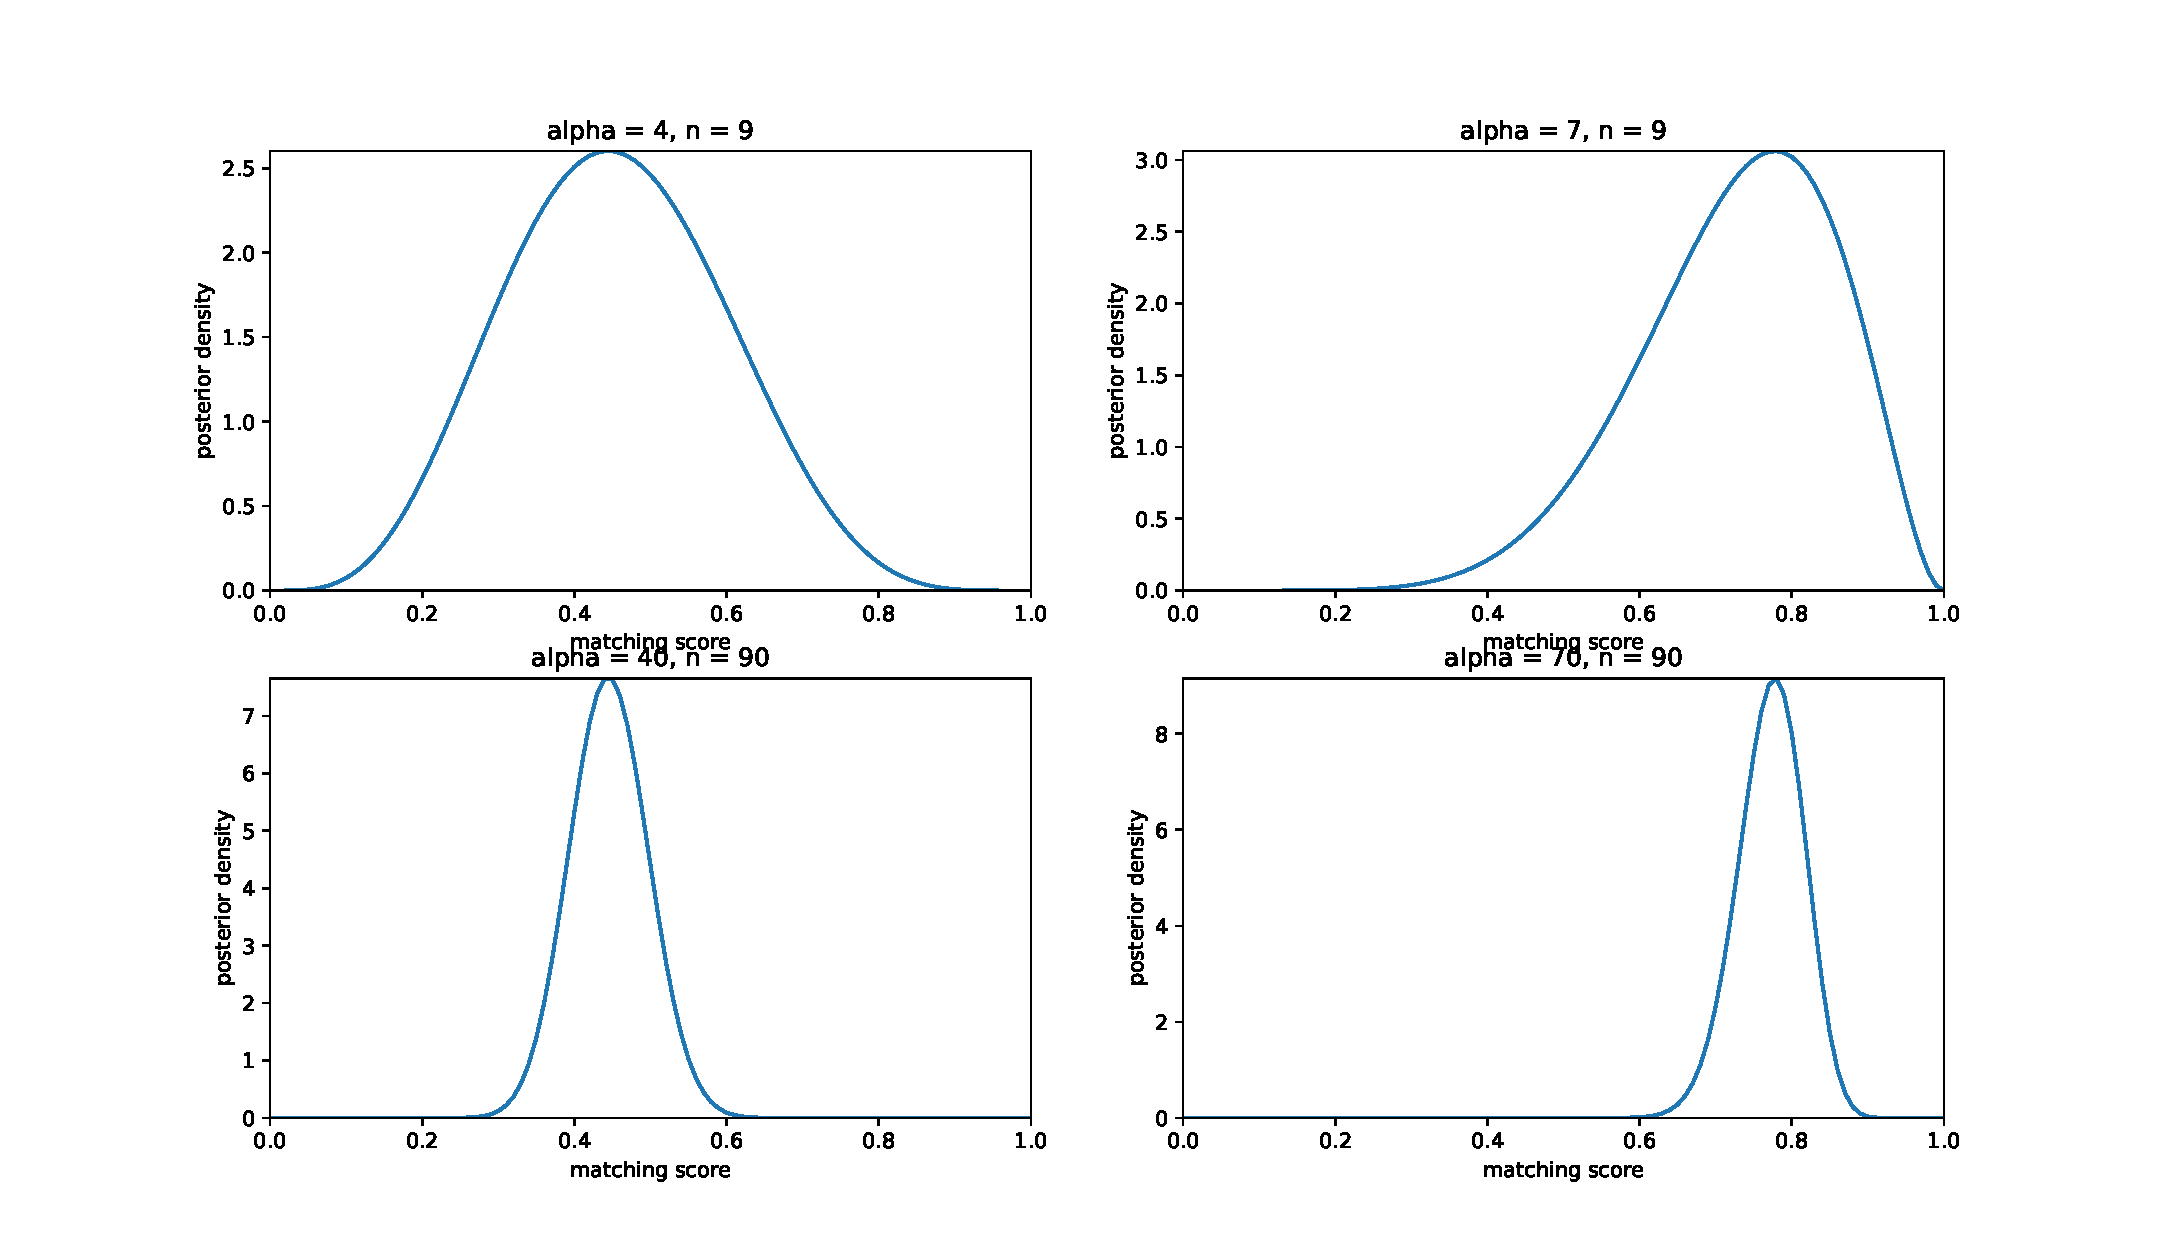
\includegraphics[width = \linewidth]{posteriors.pdf}
  \end{center}
\end{frame}

\begin{frame}{Posterior distributions:}
  \begin{center}
  \begin{minipage}{0.45\linewidth}
  \begin{exampleblock}{$\alpha=4, n=9$}
    \begin{tabular}{|l|l|}
      \hline
      $I$ & $P(\Phi \in I)$\\
          $[0, 0.1]$ & $0.0016$\\
          $[0.1, 0.2]$ & $0.0312$\\
          $[0.2, 0.3]$ & $0.1175$\\
          $[0.3, 0.4]$ & $0.2166$\\
          $[0.4, 0.5]$ & $0.2562$\\
          $[0.5, 0.6]$ & $0.2107$\\
          $[0.6, 0.7]$ & $0.1189$\\
          $[0.7, 0.8]$ & $0.0410$\\
          $[0.8, 0.9]$ & $0.0062$\\
          $[0.9, 1.0]$ & $0.0001$\\
          \hline
    \end{tabular}
  \end{exampleblock}
  \end{minipage}
  \begin{minipage}{0.45\linewidth}
    \begin{exampleblock}{$\alpha=40, n=90$}
      \begin{tabular}{|l|l|}
      \hline
      $I$ & $P(\Phi \in I)$\\
      $[0, 0.1]$ & $0.0000$\\
      $[0.1, 0.2]$ & $0.0000$\\
      $[0.2, 0.3]$ & $0.0017$\\
      $[0.3, 0.4]$ & $0.1880$\\
      $[0.4, 0.5]$ & $0.6630$\\
      $[0.5, 0.6]$ & $0.1458$\\
      $[0.6, 0.7]$ & $0.0014$\\
      $[0.7, 0.8]$ & $0.0000$\\
      $[0.8, 0.9]$ & $0.0000$\\
      $[0.9, 1.0]$ & $0.0000$\\
      \hline
    \end{tabular}
    \end{exampleblock}
  \end{minipage}
  \end{center}
\end{frame}
  
\end{document}
